
\begin{frame}
[plain]
  \titlepage
\end{frame}
%\begin{frame}
%{Содержание}
%  \tableofcontents
%  % You might wish to add the option [pausesections]
%\end{frame}
\section{Введение}

\begin{frame}{Main task of protein design}
    \centering
\tikzstyle{block} = [rounded corners=10, rectangle, text centered, node distance=2.0cm ,   text width = 3cm, minimum height = 2em]
    \begin{tikzpicture} %[remember picture,overlay]
        \node (1) [block,draw,text width = 5.5cm,]  { \centering \Large Sequence \small \newline
MTDDKDVLRD VWFGRIPTCF TLYQDEITER EAEPYYLLLP RVSYLTLVTD };
        \node (2) [ block,draw, right of=1,  text width = 3.5cm, xshift=5cm] {\centering \Large Structure \newline
            \includegraphics[height=3cm]{prot2}};
     \draw[white,->,thick,>=stealth']  (1.south) --++(0,-4em)  -|  (2.south) ;
     \draw[white,->,thick,>=stealth']  (2.north) --++(0,2em)  -|  (1.north) ;
     %(1.south) -- ([xshift=1cm]1.south)  |-  (2.south);
 %    \draw[magenta!50!black,->,thick,>=stealth'] (1.south) -- (2.north) ;
%     \draw[magenta!50!black,->,thick,>=stealth',xshift=0.5cm] (2.north) -- (1.south) ;
     %\draw[magenta!50!black,->,thick,>=stealth'] (2.south) -- (3.north) ;
     \end{tikzpicture}
\end{frame}

\begin{frame}
{Основные проблемы:}{}
 \begin{itemize}
  \item
	  Монте-Карло: 100 а.к. 3\textsuperscript{N} степеней свободы, получаем 10\textsuperscript{48} конформаций.
\vspace{0.2cm}
  \item
	  \textbf{Парадокс Левинталя:} "Промежуток времени, за который полипептид приходит к своему скрученному состоянию, на много порядков меньше, чем если бы полипептид просто перебирал все возможные конфигурации".
\vspace{0.2cm}
  \item
Для решения разумно использовать накопленные знания для моделирования.
 \end{itemize}
\end{frame}
\begin{frame}
{Последовательность-структура}{}
	\textbf{Причины парадокса Левинталя:}
 \begin{itemize}
\item
Теоретические модели, не соответствуют тому, что природа старается оптимизировать;	  
\vspace{0.2cm}
\item
В ходе эволюции были отобраны только те белки, которые легко сворачиваются;	  
\vspace{0.2cm}
\item
белки могут сворачиваться разными путями, не обязательно следуя глобально оптимальному пути.
	\vspace{.5cm}
\item
Считается, что структура определяется последовательностью, но иногда нужны другие факторы.
\item
Структура более консервативна чем последовательность
 \end{itemize}
\end{frame}
\begin{frame}
{Сравнительное моделирование}{}
 \begin{itemize}
  \item
	  Зачем искать конформации если можно представить, что при подобии последовательностей подобны и структуры.
\vspace{0.2cm}
  \item
	  Надо оценить насколько вероятно, что отличие в последовательности может привести изменению способа укладки цепи.
\vspace{0.2cm}
  \item
	  Надо отфильтровать ошибки полученные при определении структуры.
  \end{itemize}
\end{frame}
\begin{frame}
{Известные структуры и последовательности}{}
 \begin{itemize}
  \item
	  Сейчас известно порядка 1.6*10\textsuperscript{5} структур уникальных белков. 
\vspace{0.2cm}
  \item
	  UniProt это 562 000 белоков.
\vspace{0.2cm}
  \item
	  Для 50\% последовательностей можно предсказать способ укладки.
  \end{itemize}
\end{frame}


\begin{frame}{Степень идентичности и сравнительное моделирование}{}
    \centering
\begin{tikzpicture}
     \node [rectangle, left color=red!30!white, right color=green!30!white, anchor=center, minimum width=0.5\paperwidth, minimum height=1.0cm,
     text=NordBlack] (box) at
     (current page.center)
     { \Large 
      0    \hspace{3.5cm} 30    \hspace{3.5cm} 60    \hspace{3.5cm}    100
     };
\end{tikzpicture}
        \begin{columns}
                \begin{column}{0.3\textwidth}
    \centering
                        \includegraphics[width=.7\textwidth]{comp-scale-1.png} \\
            Фолд, мотивы
                \end{column}
                \begin{column}{0.3\textwidth}
    \centering
                        \includegraphics[width=.7\textwidth]{comp-scale-2.png} \\
            MR, Мутагенез
                \end{column}
                \begin{column}{0.3\textwidth}
    \centering
                        \includegraphics[width=.7\textwidth]{comp-scale-3.png} \\
            Докинг
                \end{column}
        \end{columns}
    \vspace{1cm}
                        \footnotesize{Sali,A. \& Kuriyan,J. Trends Biochem. Sci. 22, M20–M24 (1999)}
\end{frame}


\section{Сравнительное моделирование}
\begin{frame}
{Как это реализовать?}
	\begin{itemize}
\item
Надо найти белок заготовку с известной структурой.
\item
Построить первичное выравнивание.
\item
Улучшить выравнивание. 
\item
Построить ход основной цепи.
\item
Моделирование петель
\item
Достроить/моделировать положение боковых радикалов
\item
Проверка модели
   \end{itemize}
\end{frame}
\begin{frame}
{Поиск белка заготовки}
	\begin{itemize}
		\item 
Поиск по PDB с помощью:
\begin{itemize}
	\item
Blast
    \item 
Psi-Blast
    \item
Методов распознавания упаковки
\end{itemize}
\vspace{.5cm}
\item
Используя биологическую информацию.
\item
Функциональное аннотирование в базах данных.
\item
Используя информацию об активных  сайтах, или мотивы.
\end{itemize}
\end{frame}
\begin{frame}
[fragile]{Улучшение выравнивания}
	\small{
\begin{verbatim}
 1   2   3   4   5   6   7   8   9   10  11  12  13  14
\end{verbatim}
\vspace{-0.5cm}\color{green}\begin{verbatim}
PHE ASP ILE CYS ARG LEU PRO GLY SER ALA GLU ALA VAL CYS \end{verbatim}
\vspace{-0.5cm}\color{red}\begin{verbatim}
PHE ASN VAL CYS ARG THR PRO --- --- --- GLU ALA ILE CYS \end{verbatim}
\vspace{-0.5cm}\color{blue}\begin{verbatim}
PHE ASN VAL CYS ARG --- --- --- THR PRO GLU ALA ILE CYS \end{verbatim}
}
\begin{center}
		\includegraphics[width=0.4\textwidth]{ali.png}  \\
		Из книги ”Professional Gambling” от Gert Vriend 
\end{center}
\end{frame}
\begin{frame}
{Качество белка заготовки}
	\begin{itemize}
		 \item 
			 Выбор качественного белка заготовки очень важен.
		 \item
			 Лучший вариант не обязательно обладает лучшей степенью идентичности.
			 \begin{itemize}
		        \item
			  Белок 1: ID 93\%, 3.5 ангстрема разрешение. Хуже.
		        \item
			  Белок 2: ID 90\%, 1.5 ангстрема разрешение. Лучше!
		     \end{itemize}
	\end{itemize}
\begin{tikzpicture}[xscale=1.0,yscale=1.0]
    %% Pot energy plot
  \begin{axis}[height=5cm,width=11cm,
    xmin=0,xmax=400,ymin=0, ymax=100,
    tick label style={font=\footnotesize},label style={font=\small},
%hide x axis, hide y axis,
xlabel={Длина белка, а.о.}, ylabel={Идентичность,\%}]
   \addplot+[raw gnuplot, draw=red, mark=none,
   thick,domain=1:300,smooth,fill=red!20!white]
   {100*(0.97^(x-20))+20}\closedcycle;
   \node at (axis cs:350,25) {\includegraphics[width=0.17\textheight]{1a.png}};
   \node at (axis cs:350,50) {\includegraphics[width=0.17\textheight]{2a.png}};
   \node at (axis cs:350,75) {\includegraphics[width=0.17\textheight]{2a.png}};
   \node at (axis cs:200,60) {Приемлемо};
   \node at (axis cs:75,15) {Неприемлемо};
  \end{axis}
\end{tikzpicture}
\end{frame}
\begin{frame}
{Если структура белка заготовки получена ЯМР}
	\begin{itemize}
		\item
			 Определимся какие области определены лучше. 
		 \item
			  Соотнесём с выравниванием.
		  \item
			   Если низкая гомология выпадает на “подвижные” области, то структура подходит.
	\end{itemize}
	\begin{center}
	\includegraphics[width=0.9\textheight]{nmr.png}
	\end{center}
\end{frame}
\begin{frame}
{Качество заготовки, Рамачандран}
		 \begin{columns}
		\begin{column}{0.5\textwidth}
			\begin{center}
			\includegraphics[width=0.6\textheight]{ram1.png}\\
			РСА, хорошая структура.
			\end{center}
		\end{column}
		\begin{column}{0.5\textwidth}
			\begin{center}
			\includegraphics[width=0.6\textheight]{ram2.png}\\
           ЯМР, сомнительные данные.
			\end{center}
		  \end{column}
		 \end{columns}
\end{frame}
\begin{frame}
{Построение остова}
\begin{itemize}
	\item
Генерируем координаты остова моделируемого белка для остатков из выравненных областей.
\item
Не обязательно использовать координаты, могут подойти дистанционные ограничения.
\item
Большинство исследователей предпочитают Modeller. Modeller использует дистанционные ограничения. 	   
\end{itemize}
\end{frame}
\begin{frame}
{Моделирование петель}
	\begin{itemize}
		\item
			Эмпирическое моделирование:
			\begin{itemize}
				\item
					Поиск подходящего фрагмента по PDB 
				\item
					Использовать базы данных (LIP, etc..)
			\end{itemize}
 		         \item
					 Молекулярная механика.
				 \item
					 Монте-Карло.
				 \item
					 Rosetta:
					 \begin{itemize}
						 \item
			 Поиск фрагментов близких по последовательности.
						 \item
			 Комбинирование результатов поиска с помощью Монте-Карло.
					 \end{itemize}
					 \vspace{1.0cm}
		  Комбинации выше перечисленных.
	\end{itemize}
\end{frame}
\begin{frame}
{Моделирование боковых радикалов}
	\begin{itemize}
		\item
			 Если идентичность последовательностей высока то можно ожидать высокую консервативность третичных контактов. 
		 \item
			  Если анализ показывает, что важные контакты консервативны то:
	\end{itemize}
	\vspace{.1cm}
	\textbf{
		Лучше оставить конформацию боковых радикалов  из заготовки чем моделировать.}
\end{frame}
\begin{frame}
{Моделирование боковых радикалов}
	\begin{itemize}
		\item
			 Конформация боковых радикалов зависит от конформации основной цепи.
		 \item
			 Существуют базы данных  ротамеров.
		 \item
			 Некоторые исследователи считают, что SCWRL метод самый удачный. 
	\end{itemize}
	\hspace{2.0cm}Это эмпирический метод  на основе теории графов. \\
	\hspace{2.0cm}\color{blue!50!white}http://dunbrack.fccc.edu/SCWRL3.php
	\color{black}
\end{frame}
\begin{frame}
{Точность моделирования боковых радикалов}
	\begin{itemize}
		\item
			 Высокая точность моделирования достигается для боковых радикалов внутри глобулы.
			 \begin{itemize}
		 \item
			 Причина: в экспериментах остатки на поверхности более подвижны.
		 \item
			 Вычислительное проще упаковать гидрофобные остатки, чем учесть полярные контакты и водородные связи с водой или с участием воды.
			 \end{itemize}
	\end{itemize}
\end{frame}
\begin{frame}
{Улучшение модели}
	\begin{itemize}
		\item
			 Методы минимизации энергии.
		 \item
			 Моделирование молекулярной динамики (оптимизация гидрофобики)
		 \item
			 Моделирование Монте-Карло.
		 \item
			 Любой известный подход для оптимизации структуры.
	\end{itemize}
\end{frame}
\begin{frame}
{Ошибки}
	\begin{itemize}
		\item
			Обычно  ошибки не исправляются на последующих этапах моделирования.
			\begin{itemize}
		\item
			Хорошее выравнивание не исправит плохой выбор белка заготовки.
		\item
			Хорошее моделирование петель не исправит плохое выравнивание.
			\end{itemize}
		\item
			При обнаружении ошибки необходимо повторять некоторые этапы.
	\end{itemize}
\end{frame}
\begin{frame}
{Проверка}
	\begin{itemize}
		\item
			 Большинство программ для моделирования по гомологии выдают правильные значения для связей и валентных  углов.
		 \item
			  Карта Рамачандрана в большинстве случаев для модели выглядит также, как для белка заготовки
		  \item
			   Проверка на ориентацию или положение заряженных остатков может быть полезна.
		   \item
			    Использование любых экспериментальных данных:
				\begin{itemize}
			\item
				Остатки активного центра.
			\item
				Места модификаций.
			\item
				Места контактов.
				\end{itemize}
	\end{itemize}
	\vspace{0.5cm}	
				ProQ сервер оптимизирован на поиск правильной модели а не нативной структуры.
\end{frame}
\begin{frame}
{Ресурсы для гомологичного моделирования}
	\begin{itemize}
		\item
			 Modeller
			 \vspace{.5cm}
		 \item	 
			 SwissModel
			 \vspace{.5cm}
		 \item
			 Eva-CM
			 \vspace{.5cm}
		 \item
			 Nest
			 И т.д.
	\end{itemize}
\end{frame}

\section{Моделирование \protect\textit{Ab initio}}
\begin{frame}
{Предсказание структуры белка \textit{Ab initio} }
	\begin{itemize}
		\item
			 Теоретически можно использовать молекулярную динамику.
		 \item
			 Моделирование отжига, как в МД так и в Монте-Карло. 
		 \item
			 На основе фрагментов, Rosetta
	\end{itemize}
\end{frame}
\begin{frame}
{\textit{Ab initio}, Rosseta}
	\begin{itemize}
		\item
			Метод использует информацию о предсказании вторичной структуры 
		\item 
			Сравниваем фрагменты от 3 до 9 остатков с библиотекой известных структур. Строим эти фрагменты.
		\item 
			Соединяем эти фрагменты и используем Монте-Карло для оптимизации третичной структуры. 
	\end{itemize}
			\begin{figure}
		\includegraphics[width=0.6\textwidth]{rosetta.png}  
			\end{figure}
\end{frame}
\begin{frame}
{Ab initio, Rosseta}	 
	\begin{itemize}
		\item
			 Для определения хорошей конформации использую специальные потенциалы, которые делают модель похожей на нативную
		 \item 
			  Что можно использовать:
			  \begin{itemize}
			  \item
			  Потенциалы для третичных  контактов
 		      \item 
			  Гидрофобные потенциалы
		      \item
			  Потенциал для уменьшения радиуса вращения молекулы
		  \item
			  Водородные связи и т.д.
	  \end{itemize}
			   Можно добавить знание об дисульфидных мостиках, местах связывания катионов металлов и т.д.
	\end{itemize}
\end{frame}

\section{Threading — протягивание нити}

\begin{frame}
{Threading — протягивание нити}
	\begin{itemize}
		\item
			 Сравниваем последовательность со всеми известными способами укладки.
		 \item
			 Используем потенциалы для определения тенденций в известных  способах укладки.
			 \begin{itemize}
				 \item
			 Каждую аминокислоту из модели помещаем в позиции белков разных укладок
		 \item
			 Определяем как хорошо эта аминокислота подходит белку заготовке на основе парных взаимодействий
		 \item
			 Но основе суммарного результата определяем белок заготовку.
			 \end{itemize}
	\end{itemize}
\end{frame}
\begin{frame}
{Threading — протягивание нити}
	\begin{center}
		\includegraphics[width=0.5\textwidth]{threading.png}  
	\end{center}
\end{frame}
\begin{frame}
{Threading — недостатки}
	\begin{itemize}
		\item
			 Взаимодействия в белке не всегда описываются парными контактами.
		 \item
			 Потенциалы часто основываются на профилях последовательностей.
	\end{itemize}
	\vspace{1.0cm}
	Есть гибридные методы Rosseta/Threading: I-Tasser
\end{frame}
\section{Распознавание укладки}

\begin{frame}
{Распознавание укладки, Phyre2}
\centering
		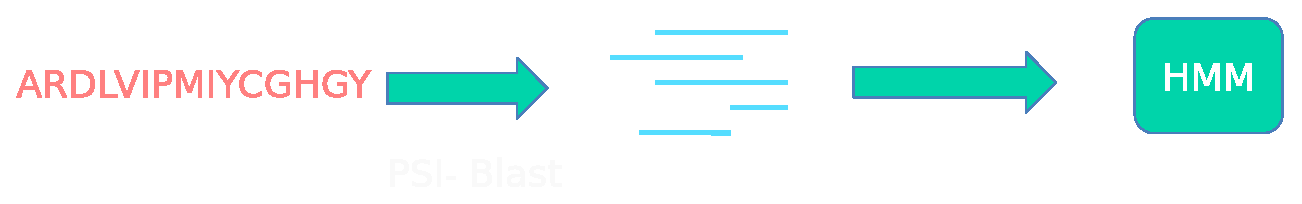
\includegraphics[width=0.8\textwidth]{phyre3.eps}  
\end{frame}
\begin{frame}
{Phyre2}
\centering

		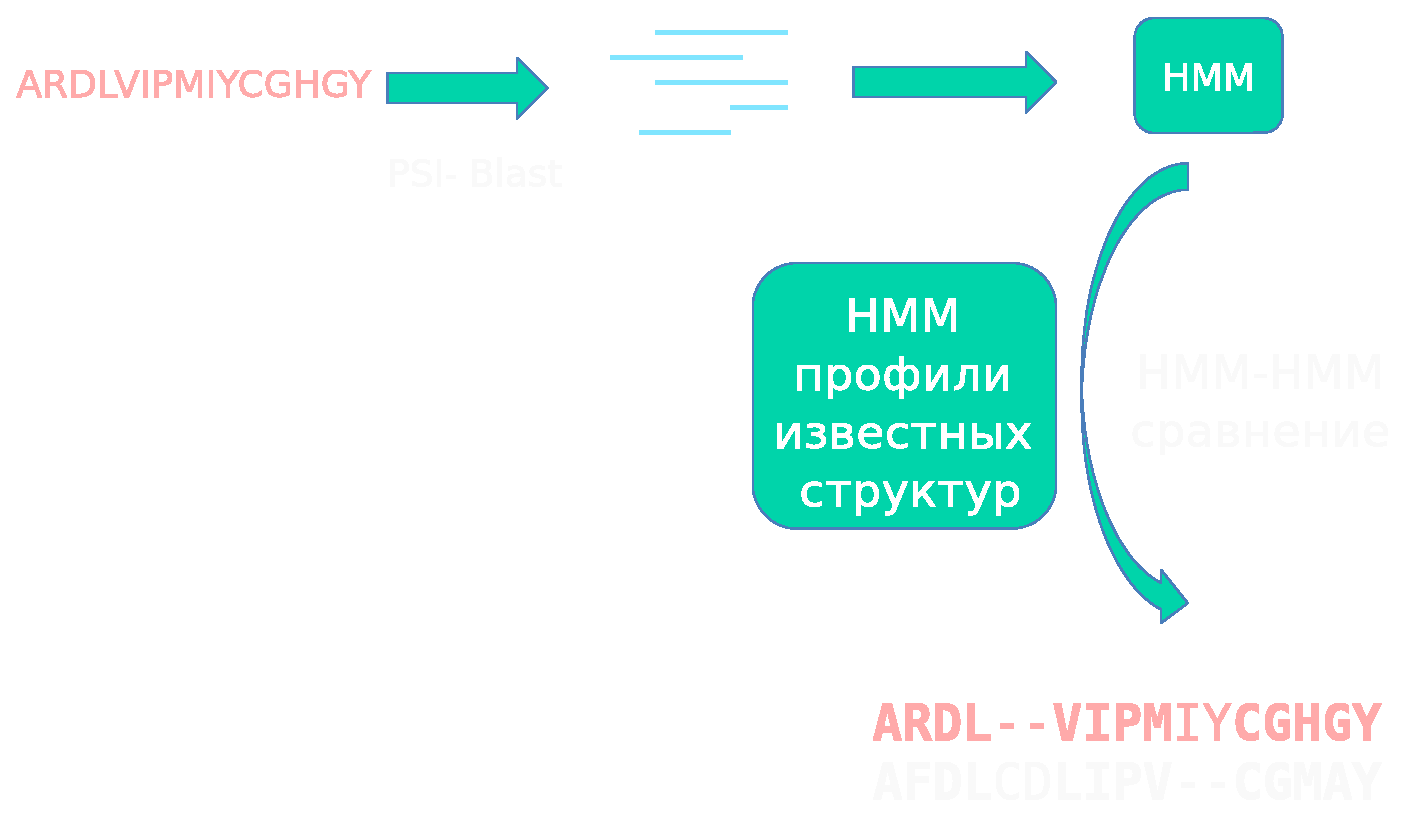
\includegraphics[width=0.7\textwidth]{phyre4.eps}  
\end{frame}
\begin{frame}
{Phyre2}
\centering
		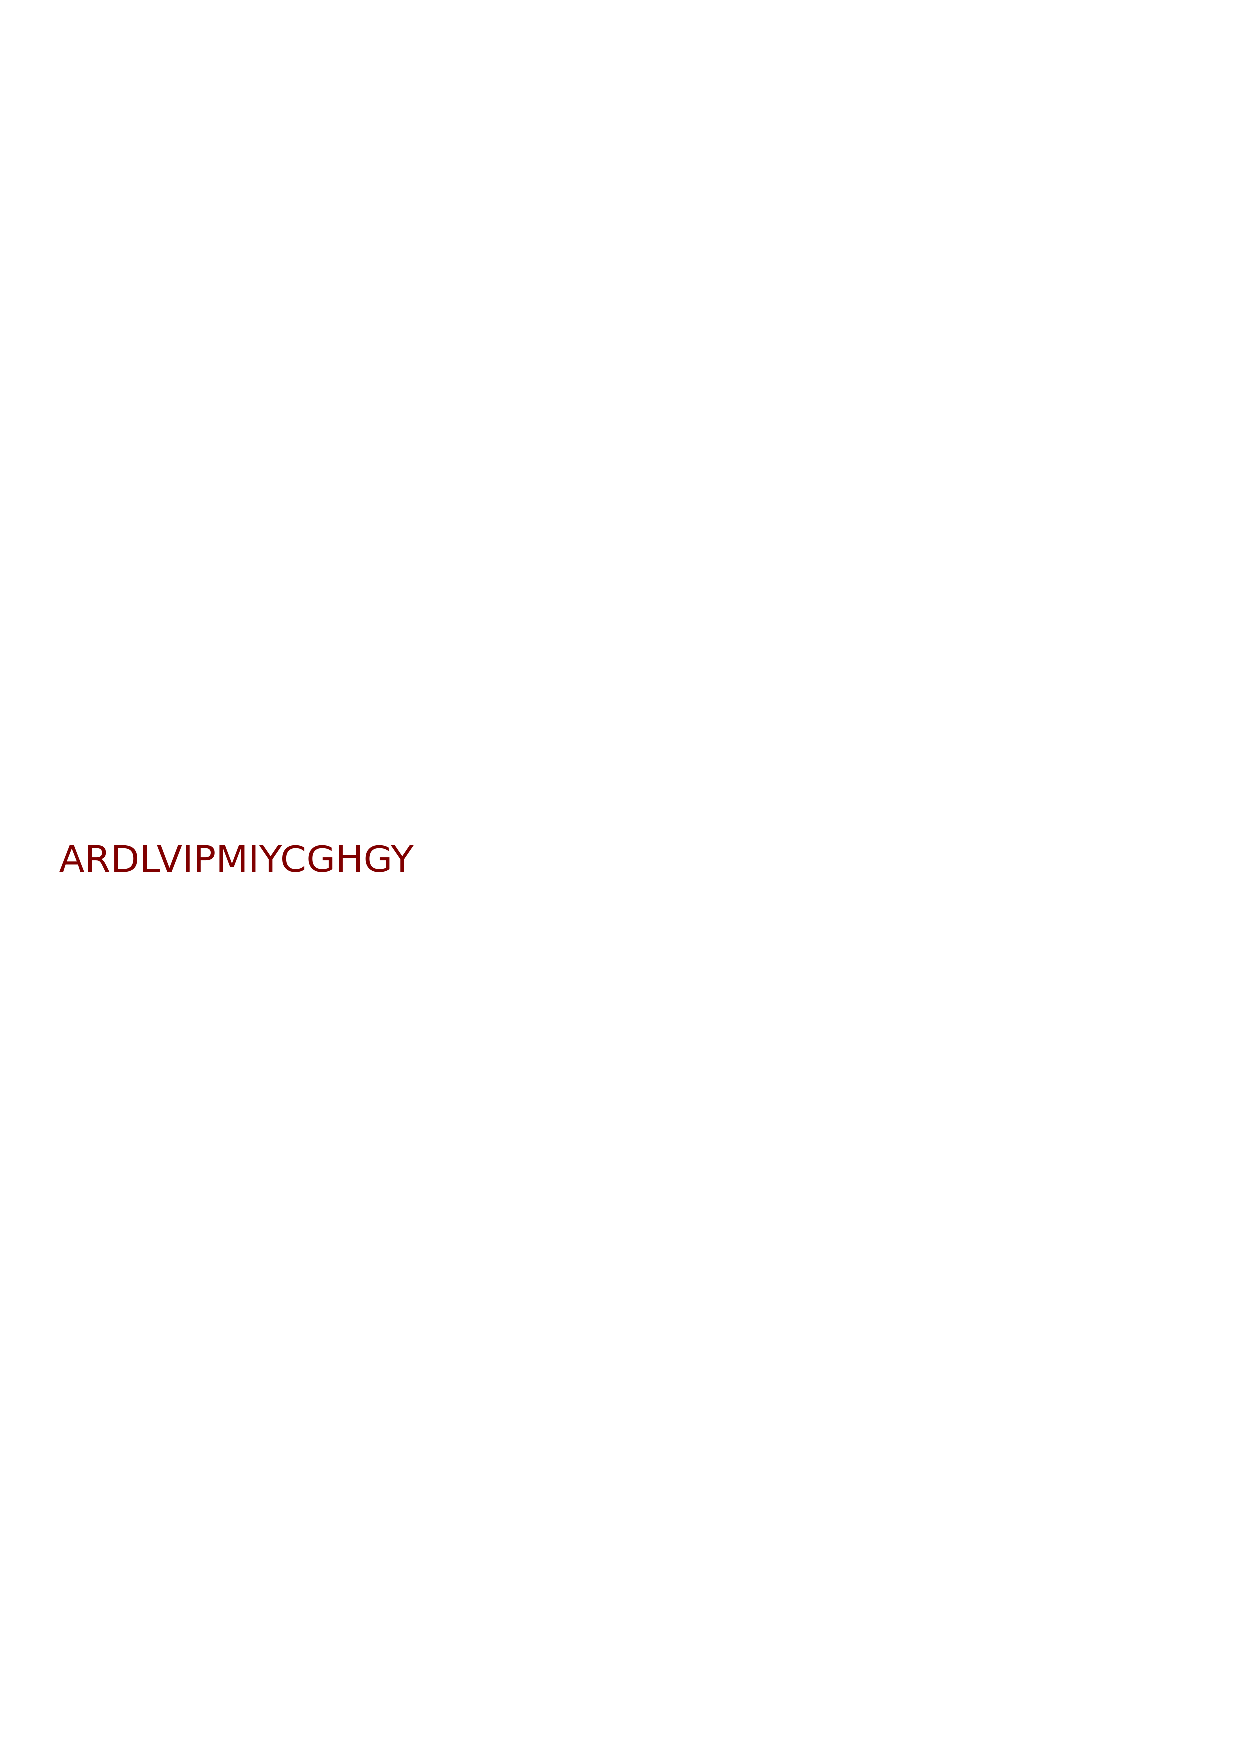
\includegraphics[width=0.7\textwidth]{phyre5.pdf}  
\end{frame}

\section{Мета серверы}
\begin{frame}
{Мета серверы}
	\begin{itemize}
		\item 
			 Сравнение разных  методов.
		 \item
			 Большинство методов предсказывают правильную укладку в первых 10-20 результатах.
			 \vspace{1.0cm}
		 \item
			 Удаление структур с высоким значением параметров модели, но  с единственной укладкой.
		 \item
			 Суперпозиция результатов, взвешивание.
		 \item
			 Часто выдают только позиции атомов остова.
	\end{itemize}
\end{frame}

\section{ML методы для предсказания структуры}

\subsection{Данные}

\begin{frame}{PDB}
    \centering
 \includegraphics[height=.7\textheight]{pdb-stat.png}
\end{frame}

\begin{frame}{UNIPROT}
    \centering
 \includegraphics[height=.7\textheight]{uniprot-stat1.png}
\end{frame}

\begin{frame}{PFAM}
    Pfam is a database of protein families that includes their annotations and multiple sequence alignments generated using hidden Markov models \\
    \centering
  \includegraphics[height=.7\textheight]{pfam}
\end{frame}


\subsection{Представление}


\begin{frame}{Разнообразие}
\centering
 \includegraphics[height=.7\textheight]{prot-features} \\
 \footnotesize 10.1016/j.patter.2020.100142
\end{frame}

\begin{frame}{Представление  последовательности}
    \begin{itemize}
        \item Естественное представление это аминокислота = целое число
        \item Можно добавить MSA, PSSM как реальное число
        \item Вторичная структура как 3 или 8 букв
        \item Данные об коэволюции
    \end{itemize}
\end{frame}

\begin{frame}{Экстракция представлений}
    \begin{itemize}
        \item NLP алгоритмы:  Word2Vec, Doc2Vec, BioVec, ProtVec
        \item Неперекрывющиеся трипептиды  
        \item mLSTM (RNN), фиксированое описание для пептидов
        \item BERT и GPT3 хорошо сработали для предсказания вторичной структуры
        \item AE и VAE были удачно применены для связи последовательности со стабильностью
    \end{itemize}
\end{frame}

\begin{frame}{Представление структуры}
    \begin{itemize}
        \item Прямое использование координат атомов затруднительно
        \item Voxels, 3D сетка окружения для СNN
        \item Торсионные углы, малые изменения сильно меняют структуру
        \item Попарные растояния или карты контактов
        \item Графы для GNN, можно отделить ферменты от белков, предсказания интерфейсов
        \item Представление поверхности, MASIF
    \end{itemize}
\end{frame}

\begin{frame}{Оценочные функции и силовые поля}
    \begin{itemize}
        \item ММ Силовые поля достаточно хороши для стандартных  взаимодействий
        \item ML используется для внедрения квантовых явлений при сохранении производительности
        \item Точность может достигать очень затратных QM методов.
        \item SchNet, ANI-1x, PhysNet
    \end{itemize}
\end{frame}


\section{Варианты NN }
\begin{frame}{Convolutional NN}
\centering
 \includegraphics[height=.7\textheight]{prot-cnn.png}\\
 \footnotesize 10.1016/j.patter.2020.100142
    \end{frame}


\begin{frame}{Recurrent NN}
\centering
 \includegraphics[height=.7\textheight]{prot-rnn.png}
    \end{frame}


\begin{frame}{Variational Auto Encoder}
\centering
 \includegraphics[height=.5\textheight]{prot-vae.png}
    \end{frame}

\begin{frame}{ Generative Adversarial Network}
\centering
 \includegraphics[height=.5\textheight]{prot-gan.png}
    \end{frame}


\section{Предсказание структуры белков}

\begin{frame}{Основная идея}
    \begin{itemize}
        \item Классические методы опираются на силовые поля и сложные протоколы
        \item Новая идея: контактирующие остатки эволюционируют вместе
        \item Нужна информация об гомологах, большие MSA
        \item RaptorX и AlphaFold
    \end{itemize}
\end{frame}

\begin{frame}{Архитектуры, растояния}
 \includegraphics[height=.7\textheight]{prot-dist-matr.png}

 \footnotesize 10.1002/prot.25810
\end{frame}

\begin{frame}{Архитектуры, end2end}
 \includegraphics[height=.7\textheight]{prot-end2end.png}

 \footnotesize 10.1016/j.cels.2019.03.006
\end{frame}

\begin{frame}
{Alphafold 1, идея}
		\includegraphics[width=0.9\textwidth]{alphafold-1-method}  
 
        \footnotesize 10.1038/s41586-019-1923-7
\end{frame}

\begin{frame}
{Alphafold 1, CASP }
		\includegraphics[width=0.9\textwidth]{alphafold-1-casp}  

        \footnotesize 10.1038/s41586-019-1923-7
\end{frame}

\begin{frame}
{Alphafold 2, метод }
\begin{itemize}
    \item Проблема: Архитектуры глубокого обучения излишне отдают предпочтение локальным взаимодействиям 
        
    \item Решение: Разработана новая архитектура глубокого обучения, основанная на внимании, для достижения самосогласованной структуры.
\end{itemize}
\begin{itemize}
%    \vspace[0.5cm]
\item Маленькие MSA
\item Алгоритм глубокого обучения для полного присутствия на протяжении всего MSA,
вместо использования функций парной коэволюции.
\end{itemize}
\end{frame}



\begin{frame}
{Alphafold 2, метод }
		\includegraphics[width=0.9\textwidth]{alphafold2-method.png}  

        \footnotesize 10.1038/s41586-021-03819-2

\end{frame}

\begin{frame}
{Alphafold 2, метод }
\centering
		\includegraphics[width=0.6\textwidth]{evoformer}  

        \footnotesize 10.1038/s41586-021-03819-2

\end{frame}



\begin{frame}{Последовательности и MSA}
    \begin{itemize}
        \item Evoformer: создание массива Nseq × Nres, который представляет собой обработанный MSA
        \item Evoformer:  Массив Nres × Nres, представляющий пары остатков (структура).
        \item Ключевыми нововведениями в блоке Evoformer являются новые механизмы обмена информацией внутри MSA и парных представлений, напрямую
            связывает  пространственные и эволюционные связи.    
        \end{itemize}
    \end{frame}


\begin{frame}{Структурный модуль}
    \begin{itemize} 
        \item Явная трехмерная структура в виде вращения и трансляции каждого остатка белка 
            (глобальные каркасы твердого тела). 
        \item  Ключевая инновация : нарушение структуры цепочки, чтобы обеспечить одновременное локальное уточнение всех частей структуры
        \item Учет непредставленных атомах боковой цепи, а также термин потери, который существенно увеличивает влияние на правильность ориентации остатков.
        \item Итеративное уточнение с использованием всей сети 
    \end{itemize}
\end{frame}


\begin{frame}{Производительность AlphaFold2}
    \large
   \begin{itemize}
      \setlength\itemsep{1em}
       \item Размер белка ограничени размером RAM GPU
       \item RTX 3090, 400 а.к., около 5 минут
    \end{itemize}
    \vspace{1cm}
    не нужно, 200 млн. моделей: https://alphafold.ebi.ac.uk/
    
\end{frame}


\begin{frame}
{Alphafold 2, результат }
		\includegraphics[width=0.9\textwidth]{alphafold2-accuracy.png}  
\end{frame}


\begin{frame}
    {Оценка сообщества}
    \begin{itemize}
    \item  прогнозирование вариантов, обнаружение карманов и построение моделей на основе экспериментальных данных. Cтруктуры, предсказанные с помощью AF2, в среднем  так же хороши, как и те, которые получены на основе экспериментальных структур. 
    \item  AF2 возвращает полное предсказание по белку, часто  содержат сегменты белка, размещение которых является неопределенным. Эта неопределенность может привести к неправильным оценкам или выявлению структурного сходства, карманов, эффектов вариантов или плохого построения модели.
    \item AF2  не очень подходит для прогнозирования структур мутированных белков. 
    \item  AF2 превосходит стандартные подходы докинге белковых молекул, не требуя даже создания стартовых белковых структур.
    \end{itemize}
    \end{frame}



\begin{frame}
{trRosetta, метод }
		\includegraphics[width=0.8\textwidth]{trrosetta-method.png}  

        \footnotesize 10.1073/pnas.1914677117
\end{frame}

\begin{frame}
{trRosetta, результат }
		\includegraphics[width=0.8\textwidth]{trrosetta-accuracy.png}  
\end{frame}

\begin{frame}
{trRosetta, дизайн }
		\includegraphics[width=0.9\textwidth]{trrosetta-desighn.png}  
\end{frame}

\section{Заключение}
\begin{frame}
{Заключение}
	\begin{itemize}
		\item
			 Суть современного моделирования белков - эмпирическая
		 \item
			 Чем больше известной информации используется при моделировании тем точнее модель.
		 \item
			 Каждый метод имеет недостатки.
		 \item
			 Критический анализ модели позволяет выявить ошибки и улучшить модель.
	\end{itemize}
\end{frame}

			
%\begin{frame}
%{Функция не сдачи праков:}
%	\begin{center}
%		\input{/tmp/jopa.tex}
%    \setlength{\fboxsep}{1pt}
%     \fcolorbox{black}{white}{ 
%		 \includegraphics[width=1.0\textheight]{/tmp/jopa.png}
%	 }
%	\end{center}
%\end{frame}



			 
	


